\begin{pastexam}[label={px:ncku-114-ee-ds-18}]{成大電機所 114 學年度 簡答題第 2 題}
（問答）

(10 PTs) Given a graph shown in Fig 2, please answer the following questions:

a) which are the articulation points, and

b) the biconnected components of the graph.

\begin{center}
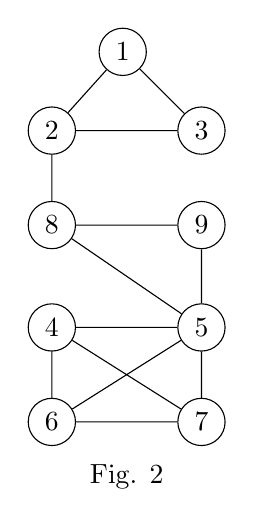
\begin{tikzpicture}[v/.style={draw,circle,minimum size=6mm,inner sep=0pt}]
  \node[v] (1) at (0.9,0) {1};
  \node[v] (2) at (0,-1) {2};
  \node[v] (3) at (1.9,-1) {3};
  \node[v] (8) at (0,-2.2) {8};
  \node[v] (9) at (1.9,-2.2) {9};
  \node[v] (4) at (0,-3.5) {4};
  \node[v] (5) at (1.9,-3.5) {5};
  \node[v] (6) at (0,-4.7) {6};
  \node[v] (7) at (1.9,-4.7) {7};
  \draw (1) -- (2) (1) -- (3) (2) -- (3) (2) -- (8) (8) -- (9) (8) -- (5) (9) -- (5)
        (4) -- (5) (4) -- (6) (4) -- (7) (5) -- (6) (5) -- (7) (6) -- (7);
  \node at (0.95,-5.4) {Fig. 2};
\end{tikzpicture}
\end{center}
\end{pastexam}

\begin{pastsoln}
答案：(a) 割點是 $2$、$8$、$5$；(b) 雙連通元件是 $\{1, 2, 3\}$、$\{2, 8\}$、$\{5, 8, 9\}$、
$\{4, 5, 6, 7\}$。

圖的邊：$(1,2), (1,3), (2,3), (2,8), (8,9), (8,5), (9,5), (4,5), (4,6), (4,7), (5,6), (5,7), (6,7)$，共
$13$ 條。

\textbf{用 DFS 的 $\mathit{low}$ 值找割點}（資結書第~23.5~節）。 從 $1$ 開始，鄰點照編號由小到大：
DFS 樹是 $1 - 2 - 3$，$3$ 回到 $2$ 之後走 $2 - 8 - 5 - 4 - 6 - 7$，$7$ 結束後回到 $5$ 再走 $5 - 9$。
後向邊是 $(3, 1)$、$(7, 4)$、$(7, 5)$、$(6, 5)$、$(9, 8)$。
\begin{center}
\begin{tabular}{c*{9}{c}}
\toprule
頂點 & 1 & 2 & 3 & 8 & 5 & 4 & 6 & 7 & 9 \\
\midrule
$\mathit{dfn}$ & 1 & 2 & 3 & 4 & 5 & 6 & 7 & 8 & 9 \\
$\mathit{low}$ & 1 & 1 & 1 & 4 & 4 & 5 & 5 & 5 & 4 \\
\bottomrule
\end{tabular}
\end{center}
（$\mathit{low}(7) = \min(8, \mathit{dfn}(4), \mathit{dfn}(5)) = 5$；$\mathit{low}(9) = \mathit{dfn}(8) = 4$，
傳給 $5$；$\mathit{low}(3) = \mathit{dfn}(1) = 1$，傳給 $2$。）

\textbf{(a) 割點。} 根 $1$ 只有一個子節點 $2$，不是割點。 非根的 $u$ 若有子節點 $w$ 使
$\mathit{low}(w) \ge \mathit{dfn}(u)$ 就是割點：
\begin{itemize}
\item $2$：子節點 $8$ 的 $\mathit{low} = 4 \ge 2$，是割點（子節點 $3$ 的 $\mathit{low} = 1 < 2$）。
\item $8$：子節點 $5$ 的 $\mathit{low} = 4 \ge 4$，是割點。
\item $5$：子節點 $4$ 的 $\mathit{low} = 5 \ge 5$，是割點（子節點 $9$ 的 $\mathit{low} = 4 < 5$）。
\item $3$、$4$、$6$、$7$、$9$：$3, 7, 9$ 是葉；$4$ 的子節點 $6$ 有 $\mathit{low} = 5 < 6$；$6$ 的子節點
$7$ 有 $\mathit{low} = 5 < 7$。 都不是。
\end{itemize}
割點是 $\{2, 5, 8\}$。 直接看圖也對得上：拿掉 $2$，$\{1, 3\}$ 斷開；拿掉 $8$，上面的 $\{1, 2, 3\}$
和下面斷開；拿掉 $5$，$\{4, 6, 7\}$ 和 $\{8, 9\}$ 斷開。

\textbf{(b) 雙連通元件}（資結書第~23.6~節），在割點處切開：
\begin{itemize}
\item $\{1, 2, 3\}$：邊 $(1,2), (1,3), (2,3)$，三角形。
\item $\{2, 8\}$：邊 $(2,8)$，橋。
\item $\{5, 8, 9\}$：邊 $(8,9), (8,5), (9,5)$，三角形。
\item $\{4, 5, 6, 7\}$：邊 $(4,5), (4,6), (4,7), (5,6), (5,7), (6,7)$，四個點兩兩相連（$K_4$）。
\end{itemize}
$3 + 1 + 3 + 6 = 13$ 條邊剛好分完，每條邊恰屬一個元件；割點 $2, 8, 5$ 各屬兩個元件。
\end{pastsoln}
